% 基礎数学 第03回 指数関数（CC BY-SA 4.0）
\documentclass[aspectratio=169]{beamer}
\usepackage{lfs-slides}
\lfscourse{基礎数学}

\title{指数関数}
\subtitle{基礎数学 第03回}
\author{}
\date{}

\begin{document}

\begin{frame}
  \titlepage
\end{frame}

\begin{frame}{今日のねらい}
  \lfsmessage{指数関数 ＝「同じ倍率でくり返し変わる量」}
  \medskip
  \begin{itemize}
    \item 前回：三角関数 ＝「くり返す」現象（波・回転）
    \item 今回：「1時間ごとに2倍」「3時間ごとに半分」のような現象
    \item 指数を 0・負の数・分数・実数へ広げる
    \item 指数関数 $y = a^x$ のグラフと性質
    \item 工学では：複利と減衰（半減期）
  \end{itemize}
\end{frame}

\section{指数法則}

\begin{frame}{指数法則}
  \lfsmessage{掛ける個数を数えれば、法則が見える}
  \begin{columns}[c]
    \column{0.5\textwidth}
      \[
        a^3 \times a^2 = \underbrace{aaa}_{3} \times \underbrace{aa}_{2} = a^{5}
      \]
      \[
        (a^3)^2 = a^3 \times a^3 = a^{6}
      \]
    \column{0.5\textwidth}
      \begin{block}{指数法則（$m, n$ は正の整数）}
        $a^m a^n = a^{m+n}$ \\[0.6ex]
        $\dfrac{a^m}{a^n} = a^{m-n}$ \quad （$m > n$）\\[0.6ex]
        $(a^m)^n = a^{mn}$ \\[0.6ex]
        $(ab)^n = a^n b^n$
      \end{block}
  \end{columns}
\end{frame}

\begin{frame}{0乗と負の指数}
  \lfsmessage{法則がそのまま成り立つように決める}
  \begin{columns}[c]
    \column{0.55\textwidth}
      \begin{center}
        % 指数を1減らすごとに値が半分になる図：2^3 から 2^{-2} まで（CC BY-SA 4.0）
\begin{tikzpicture}[xscale=1.1,yscale=0.42]
  \draw[->] (-0.3,0) -- (6.4,0);
  \foreach \i/\e/\v/\lab in {0/3/8/8, 1/2/4/4, 2/1/2/2, 3/0/1/1, 4/-1/0.5/\tfrac12, 5/-2/0.25/\tfrac14}{
    \ifnum\e<1 \def\barcol{red}\else \def\barcol{blue}\fi
    \fill[\barcol!55] (\i+0.15,0) rectangle (\i+0.85,\v);
    \node[above] at (\i+0.5,\v) {$\lab$};
    \node[below] at (\i+0.5,0) {$2^{\e}$};
  }
  \foreach \i in {0,...,4}{
    \draw[->,thick,black!60] (\i+0.6,-2.6) to[bend right=40] node[below=-1pt] {\scriptsize $\div 2$} (\i+1.4,-2.6);
  }
\end{tikzpicture}

      \end{center}
    \column{0.45\textwidth}
      指数を1減らすと、値は半分\\[0.5ex]
      → その続きとして
      \[
        a^0 = 1, \qquad a^{-n} = \frac{1}{a^n}
      \]
      {\small 確かめ：$a^3 \times a^{-3} = a^{0} = 1$\\
      なので $a^{-3}$ は $a^3$ の逆数}
  \end{columns}
\end{frame}

\begin{frame}{計算例：法則で整理してから値を出す}
  \begin{align*}
    2^5 \times 2^{-3} &= 2^{5 + (-3)} = 2^2 = 4 \\[0.5ex]
    (3^2)^{-1} &= 3^{-2} = \frac{1}{3^2} = \frac{1}{9} \\[0.5ex]
    10^3 \div 10^5 &= 10^{3 - 5} = 10^{-2} = \frac{1}{100}
  \end{align*}
  \begin{alertblock}{よくある間違い}
    $2^{-2} = -4$ ではない \quad → \quad $2^{-2} = \dfrac{1}{4}$（負の指数は「逆数」）
  \end{alertblock}
\end{frame}

\begin{frame}{演習①}
  \lfsmessage{ワークシート 問1}
  \bigskip
  \begin{itemize}
    \item 指数法則・0乗・負の指数の計算
    \item 先に指数を整理してから、値を出す
  \end{itemize}
\end{frame}

\section{有理数・実数の指数}

\begin{frame}{累乗根と有理数の指数}
  \lfsmessage{$a^{\frac{m}{n}} = \sqrt[n]{a^m}$}
  \begin{columns}[t]
    \column{0.5\textwidth}
      \begin{block}{累乗根}
        $n$ 乗すると $a$ になる正の数を $\sqrt[n]{a}$ と書く\\[0.5ex]
        例：$2^3 = 8$ なので $\sqrt[3]{8} = 2$
      \end{block}
    \column{0.5\textwidth}
      \begin{block}{法則から決まる}
        $\left(a^{\frac13}\right)^3 = a^{\frac13 \times 3} = a^1 = a$\\[0.5ex]
        なので $a^{\frac13} = \sqrt[3]{a}$
      \end{block}
  \end{columns}
  \medskip
  \[
    27^{\frac23} = \left(\sqrt[3]{27}\right)^2 = 3^2 = 9
  \]
\end{frame}

\begin{frame}{実数の指数へ}
  \lfsmessage{$2^{\sqrt{2}}$ も「近づいていく値」として決まる}
  \begin{columns}[c]
    \column{0.45\textwidth}
      \begin{center}
        \begin{tabular}{ll}
          \toprule
          $x$ & $2^x$ \\
          \midrule
          $1.4$ & $2.639\ldots$ \\
          $1.41$ & $2.657\ldots$ \\
          $1.414$ & $2.664\ldots$ \\
          $1.4142$ & $2.665\ldots$ \\
          \bottomrule
        \end{tabular}
      \end{center}
    \column{0.55\textwidth}
      \begin{itemize}
        \item $1.4 = \frac{14}{10}$ などは有理数なので $2^{1.4}$ は計算できる
        \item $x$ を $\sqrt{2} = 1.41421\ldots$ に近づけると、$2^x$ は $2.665\ldots$ に近づく
        \item これで、すべての実数 $x$ で $2^x$ が決まる
      \end{itemize}
  \end{columns}
\end{frame}

\begin{frame}{演習②}
  \lfsmessage{ワークシート 問2}
  \bigskip
  \begin{itemize}
    \item 分数の指数は「分母が累乗根、分子が累乗」
    \item 累乗根は、指数の形に直してから法則を使う
  \end{itemize}
\end{frame}

\section{指数関数のグラフ}

\begin{frame}{指数関数 $y = a^x$ のグラフ}
  \begin{columns}[c]
    \column{0.5\textwidth}
      \begin{center}
        % 指数関数 y = 2^x と y = (1/2)^x のグラフ（CC BY-SA 4.0）
\begin{tikzpicture}[scale=0.62]
  \draw[step=1,black!12] (-3.4,-0.4) grid (3.4,6.4);
  \draw[->] (-3.6,0) -- (3.7,0) node[right] {$x$};
  \draw[->] (0,-0.6) -- (0,6.7) node[above] {$y$};
  \foreach \t in {-3,-2,-1,1,2,3} \node[below,font=\scriptsize] at (\t,0) {$\t$};
  \node[below left,font=\scriptsize] at (0,0) {O};
  \foreach \t in {2,4,6} \node[left,font=\scriptsize] at (0,\t) {$\t$};
  \draw[very thick,blue,domain=-3.4:2.6,samples=60] plot (\x,{2^\x});
  \draw[very thick,red,domain=-2.6:3.4,samples=60] plot (\x,{2^(-\x)});
  \node[blue,right] at (2.55,5.9) {$y = 2^x$};
  \node[red,left] at (-2.55,5.9) {$y = \left(\tfrac12\right)^x$};
  \fill (0,1) circle (3pt);
  \draw[->,thin] (1.05,1.55) -- (0.12,1.05);
  \node[right,font=\small,fill=white,inner sep=1pt] at (1.05,1.55) {$(0,\,1)$};
\end{tikzpicture}

      \end{center}
    \column{0.5\textwidth}
      \lfsmessage{$a > 1$ は右上がり\\$0 < a < 1$ は右下がり}
      \begin{itemize}
        \item どちらも点 $(0,\,1)$ を通る（$a^0 = 1$）
        \item $y$ はいつも正。$x$ 軸に近づくが、交わらない
        \item 2つのグラフは $y$ 軸について対称
      \end{itemize}
  \end{columns}
\end{frame}

\begin{frame}{グラフの性質と大小比較}
  \lfsmessage{底をそろえれば、指数で比べられる}
  \medskip
  $a > 1$ のとき \quad $p < q \iff a^p < a^q$ \quad （右上がり）\\[0.5ex]
  $0 < a < 1$ のとき \quad $p < q \iff a^p > a^q$ \quad （右下がり）
  \begin{block}{例：$4$ と $\sqrt[3]{32}$ の大小}
    $4 = 2^2$，\ $\sqrt[3]{32} = 2^{\frac53}$ \quad 底 $2 > 1$ で $\dfrac53 < 2$ \quad
    よって $\sqrt[3]{32} < 4$
  \end{block}
\end{frame}

\begin{frame}{演習③}
  \lfsmessage{ワークシート 問3・問4}
  \bigskip
  \begin{itemize}
    \item 問3：グラフが通る点から、底 $a$ を読み取る
    \item 問4：底を $2$ にそろえて、指数で比べる
  \end{itemize}
\end{frame}

\section{工学では}

\begin{frame}{工学では：複利と減衰}
  \lfsmessage{一定時間ごとに同じ倍率 → 指数関数}
  \begin{columns}[c]
    \column{0.42\textwidth}
      \begin{block}{複利（年利 $5\%$）}
        100万円が $n$ 年後に $100 \times 1.05^n$ 万円\\
        10年後は約 $162.9$ 万円
      \end{block}
      \begin{block}{減衰（半減期 3 時間）}
        $m(t) = 80 \left(\dfrac12\right)^{\frac{t}{3}}$ mg
      \end{block}
      {\small 薬の血中濃度・放射性物質・コンデンサの放電なども同じ形}
    \column{0.58\textwidth}
      \begin{center}
        % 減衰（半減期 3 時間、初めの量 80）：m(t) = 80 (1/2)^{t/3}（CC BY-SA 4.0）
\begin{tikzpicture}[xscale=0.44,yscale=0.032]
  \draw[->] (0,0) -- (13,0) node[right] {$t$（時間）};
  \draw[->] (0,0) -- (0,92) node[above] {$m$（mg）};
  \foreach \t in {0,3,6,9,12} \node[below,font=\scriptsize] at (\t,0) {$\t$};
  \draw[very thick,blue,domain=0:12.5,samples=80] plot (\x,{80*0.5^(\x/3)});
  \foreach \t/\m in {0/80,3/40,6/20,9/10}{
    \draw[dashed,black!50] (\t,0) -- (\t,\m) -- (0,\m);
    \fill (\t,\m) circle (2.5pt);
    \node[left,font=\scriptsize] at (0,\m) {$\m$};
  }
\end{tikzpicture}

      \end{center}
  \end{columns}
\end{frame}

\begin{frame}{確認問題}
  \lfsmessage{確認問題（5問・10分）}
  \bigskip
  \begin{itemize}
    \item マークシートに、学籍番号と答えをマークする
    \item 計算は余白を使ってよい
  \end{itemize}
\end{frame}

\begin{frame}{まとめ}
  \begin{itemize}
    \item 指数を広げる決まりは1つ：\textbf{指数法則がそのまま成り立つように}
    \item $a^0 = 1$，\ $a^{-n} = \dfrac{1}{a^n}$，\ $a^{\frac{m}{n}} = \sqrt[n]{a^m}$
    \item $y = a^x$ は点 $(0,\,1)$ を通り、値はいつも正
    \item $a > 1$ なら増加、$0 < a < 1$ なら減少
    \item 一定時間ごとに同じ倍率で変わる量（複利・減衰）は指数関数で表す
  \end{itemize}
  \bigskip
  \lfsmessage{次回：対数関数（「何乗すれば $8$ になる？」）}
\end{frame}

\end{document}
